Skemaernes fitness er beregnet ud fra værdierne vist på figur~\ref{fitnessvalues}.

\begin{figure}[!h]
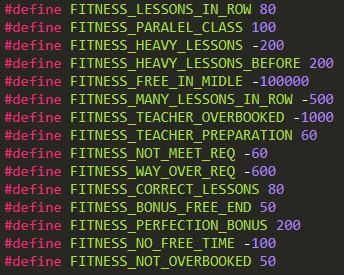
\includegraphics[scale = 2]{partials/graphics/fitness.png}
\caption{Billede over de fitness værdier skemaerne bliver tildelt, i tilfælde af at de opfylder visse parametre}
\label{fitnessvalues}
\end{figure}
De forskellige fitnessparametre kan godt give negative eller give positive værdier mere end en gang. Det vil sige at, hvis der er to steder på skemaet, hvor der er en lærer der er overbooked giver det -2000 i fitness to gange.
I denne test, undersøges det om fitnessen udregnes korrekt. De nedenstående skemaer er generet gennem softwareløsningen. De tre skemaer er alle skemaer for 7.C, de skal altså derfor alle have det samme antal af timer og de samme fag. 
I det første skema mangler 7.C to dansk lektioner, det kan ses på at perfection graden er  på 12, hvis skemaet havde opfyldt alle krav om timeantal, ville perfection graden have været 13. Udover at der mangler to dansk lektioner har dette skema også for mange af nogle lektioner. Dette kan observeres i Must have og Have, hvor fagene står i følgende rækkefølge dansk, matematik, engelsk, tysk, fysik/kemi, historie, samfundsfag, valgfag, geografi, biologi, idræt, kristendom, praktiske fag og fri timer til sidst. I det første skema er der fem fag, hvor der er for mange lektioner, navnlig engelsk, hvor der er to lektioner for meget, tysk hvor der er en lektion for meget, historie hvor der er en for meget, samfundsfag hvor der er en for meget og biologi hvor der er en for meget. Dette har negativ indflydelse på skemaet.
Skemaets positive fitness er en kombination af lessons with parallel, som er det antal af lektioner der foregår på samme tid som en af parallelklasserne og lessons with both, hvor der er mulighed for samarbejde mellem alle tre parallelklasser på en gang. Dette skema har otte lektioner, hvor det er muligt at arbejde sammen med en a parallelklasserne. Dette skema har dog ingen lektioner på sammen tid med begge parallelklasser. Derudover får dette skema mindre i fitness, ved at det har ’tunge’ fag som ligger over middag. I dette skema ligger er der otte tunge fag, som ligger efter middag. Derudover er lærerne også overbooked fire gange i dette skema, det vil sige at der er fire tilfælde, hvor en af klassens lærer, har en eller flere lektioner på samme tid. Skemaets samlede fitness er 5561. 
\begin{figure}[!h]
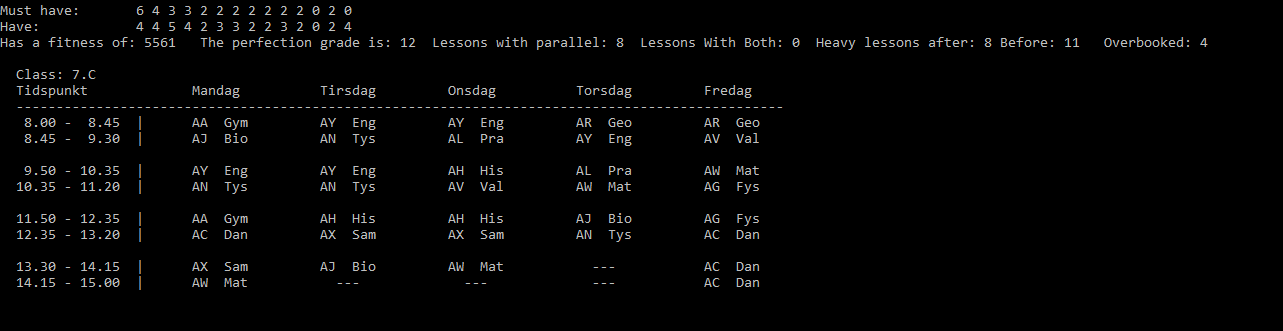
\includegraphics[width=\textwidth]{partials/graphics/fitness1.png}
\caption{Billede af et generet skema}
\label{fitness1}
\end{figure}

Det andet skema har en perfction grade på 13, alle kravene for antallet af lektioner for de forskellige fag er altså opfyldt. Der er dog tre fag hvor der er en lektion for meget, fagene for disse lektioner er samfundsfag, hvor der er en lektion for meget, geografi, hvor der er en lektion for meget og praktiske fag, hvor der er to lektioner for meget. I skemaet er der tre fælles lektioner med parallel klasserne, der er dog ingen lektioner, hvor der er mulighed for samarbejde med begge parallelklasser på samme tid. På skemaet er der syv lektioner med tunge fag over middag. Der er to steder, hvor en lærer er overbookedt. Dette skemas samlede fitness er 10341.
\begin{figure}[!h]
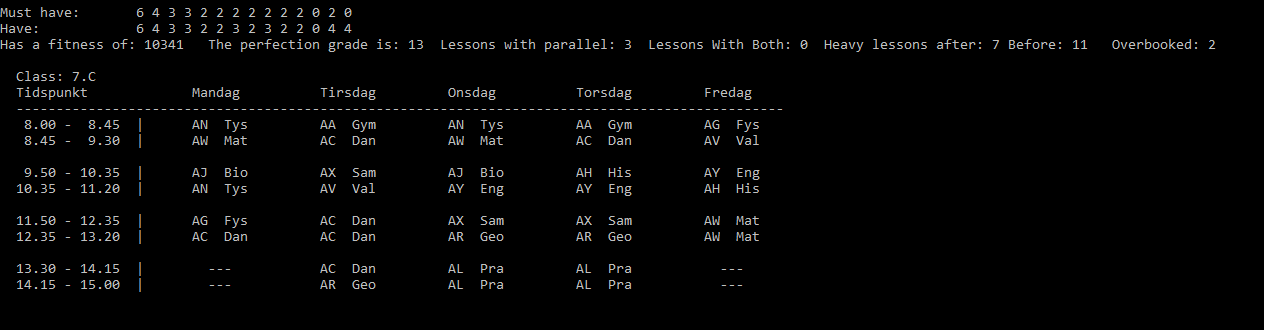
\includegraphics[width=\textwidth]{partials/graphics/fitness2.png}
\caption{Billede af et generet skema}
\label{fitness2}
\end{figure}

Perfection graden er 13 i det tredje skema, der er altså ikke for lidt lektioner af nogle fag. Der er dog tre fag hvor der er for mange lektioner. Disse fag er dansk hvor der er en lektion for meget, samfundsfag hvor der er en lektion for meget og praktiske fag hvor der er en for meget. På dette skema er der fire lektioner, hvor der er mulighed for at samarbejde med en parallelklasse i otte af skemaets lektioner, der er en lektion, hvor der er mulighed for at samarbejde med begge parallelklasser sammentidigt. På det tredje skema er der fem gange, hvor et tungt fag ligger over middag, dette er det mindste antal ud af de tre skemaer. Det forekommer ingen gang at lærerne i det tredje skema har to planlagte skemaer på samme tid. 
\begin{figure}[!h]
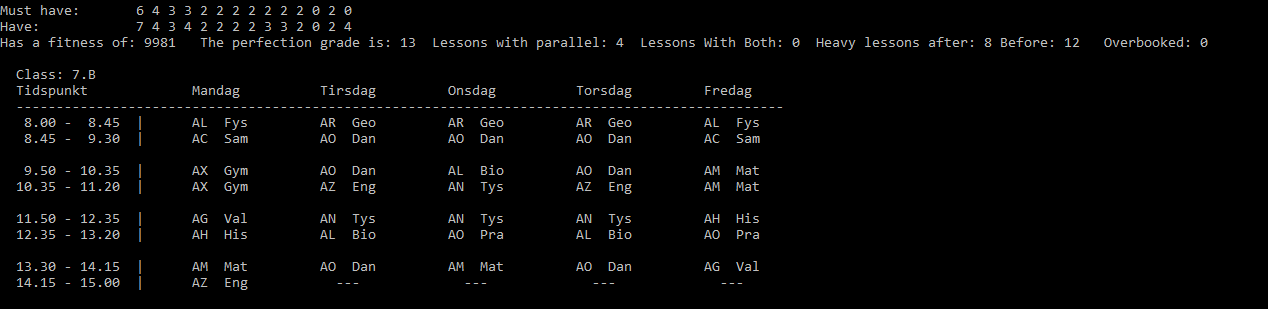
\includegraphics[width=\textwidth]{partials/graphics/fitness3.png}
\caption{Billede af et generet skema}
\label{fitness3}
\end{figure}

På tabellen med fitnessværdier, kan man se at fitnessværdien bliver trukket meget ned af have lærere der er ’overbooked,’ dette passer med at det tredje skema er det bedste da det ikke har nogle lærere der er ’overbooked’. Derudover er det også den tredje der har mindst tunge lektioner over middag, hvilket også trækker de andre to skemaer ned. Det sidste skema er også det eneste skema, hvor der er mulighed for samarbejde mellem alle parallelklasserne sammentidigt. 
Ud fra tabellen med fitnessværdierne og undersøgelsen af de tre skemaer, kan det konkluderes at fitnessfunktionen fungerer som den skal. 
